 \documentclass[12pt]{article}

\usepackage{hyperref}
\usepackage{ifxetex,ifluatex}
\ifluatex
  \usepackage{unicode-math}
  \setmainfont{Times New Roman}
  \setmathfont{XITS Math}
\else\ifxetex
  \usepackage{fontspec}
  \setmainfont{Times New Roman}
\else
  \usepackage[T1]{fontenc}
  \usepackage[utf8]{inputenc}
  \usepackage{newtxtext,newtxmath}
\fi\fi

\usepackage{sectsty}
\sectionfont{\fontsize{14}{16.8}\selectfont}
\subsectionfont{\fontsize{13}{15.6}\selectfont}

\usepackage[a4paper, left=2cm, right=2cm, top=2cm, bottom=2cm]{geometry}
\usepackage{float}
\usepackage{graphicx}
\usepackage{amsmath}
\usepackage[utf8]{inputenc}
\usepackage{enumitem}
\usepackage[portuguese]{babel}
\usepackage{indentfirst}
\usepackage{hyperref}
\hypersetup{
    colorlinks=true,
    linkcolor=blue,
    citecolor=blue,
    filecolor=magenta,
    urlcolor=cyan,
    pdftitle={Lista},
    pdfpagemode=FullScreen,
    }
\urlstyle{same}
\renewcommand\contentsname{Sumário}
\title{Trabalho Computacional: Entrega 1 \\ Modelagem Matemática do Problema de Otimização}                  % Titulo
\author{Gabriel Teixeira Lara Chaves \\ Pedro Barbosa Bahia}
     % Autores
\date{\today}                                       % Data

\def\uname{Universidade Federal de Minas Gerais}    %Universidade
\def\depart{Escola de Engenharia}                   %Departamento
\def\materia{Teoria da Decisão}
\def\turma{ELE088 - TCC}                                % Turma
\def\email{2017088182 \\ 2018019907}     % Matricula
\makeatletter
\let\thetitle\@title
\let\theauthor\@author
\let\thedate\@date
\makeatother


\begin{document}
\sloppy
\begin{titlepage}
    \centering
    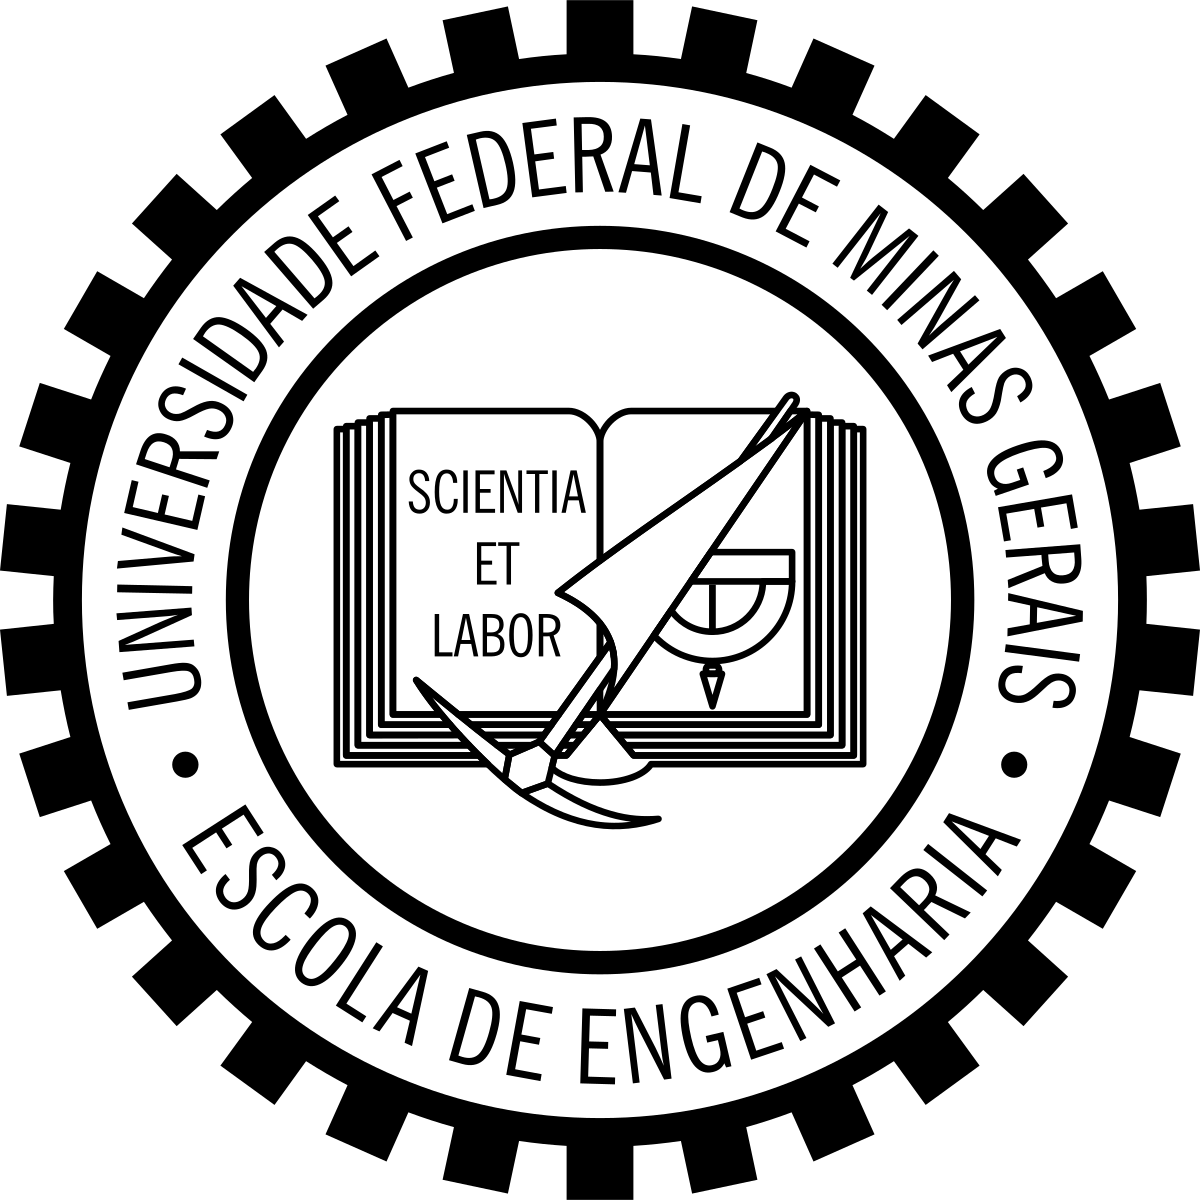
\includegraphics[scale = 0.15]{imagens/engenharia.png}\\[1.5 cm]         % Logo da Universidade
    \textsc{\LARGE \uname}\\[0.9 cm]                                % Nome da Universidade
     \textsc{\LARGE \depart}\\[0.9 cm]                              % Departamento
    \textsc{\large \materia}\\[0.5 cm]                              % Nome da Matéria
    \textsc{\large \turma}\\[0.5 cm]                                % Turma
    \rule{\linewidth}{0.2 mm} \\[0.6 cm]
    { \huge \bfseries \thetitle}\\
    \rule{\linewidth}{0.2 mm} \\[1.5 cm]
       \begin{minipage}{0.6\textwidth}
        \begin{flushleft} \large
            \emph{Aluno:}\\
            \theauthor \\
         \end{flushleft}
     \end{minipage}~
     \begin{minipage}{0.4\textwidth}
         \begin{flushright} \large
           \emph{Matrícula:} \\
            \email \\
         \end{flushright}
     \end{minipage}\\[1 cm]
    \textit{\large Professor:}\\
     \large  Lucas S. Batista\\[1 cm]
    \vfill
    {\large \thedate}\\[1 cm]

    \vfill

\end{titlepage}

\newpage

\section{Especificação do Problema}
Uma empresa possui um conjunto $\mathcal{T}$ com $n$ tarefas a serem realizadas e um conjunto $\mathcal{A}$
com $m$ agentes disponíveis. Assuma que $c_{ij}$ é o custo de atribuir a tarefa  $j\in \mathcal{T}$ ao agente
$i\in \mathcal{A}$, $a_{ij}$ é a quantidade de recursos necessários ao agente $i\in \mathcal{A}$ para realizar a tarefa
$j\in \mathcal{T}$, e $b_i$ é a disponibilidade total de recursos do agente $i\in \mathcal{A}$.



\section{Modelagem do Problema}

O problema a ser modelado é de otimização sobre variáveis lógicas onde a
variável de otimização descreve a atribuição de uma tarefa a um agente.

\subsection{Definição da Variável de Otimização}

As variável de otimização $\mathbf{x}$ é binária tal que

$$ x_{ij} = \begin{cases} 1, \text{se a tarefa $j$ for atribuída ao agente $j$}
                       \\ 0, \text{caso contrário}
            \end{cases} $$

\subsection{Função de Custo sobre Custo Total}

A função de custo $f_C$, a ser minimizada, deve quantificar o custo total de
realização de todas as tarefas.

Definimos $f_C$ como a seguir

$$ f_C(\mathbf{x}, \mathbf{c}) = \sum^{n}_{j=1}\sum^{m}_{i=1} c_{ij} x_{ij} $$

\subsection{Função de Custo sobre Diferença no Consumo de Recursos}

Definimos inicialmente uma função responsável por quantificar o consumo
total de recursos por agente $i$, denominada $CRA_i$.

$$ CRA_{i} (\mathbf{x}, \mathbf{a}) =  \sum^{n}_{j=1} a_{ij} x_{ij} $$

Em seguida construímos a função para minimização da diferença do consumo de
recursos entre o agente mais ocupado e o agente menos ocupado, $f_E$, como

$$ f_E(\mathbf{x}, \mathbf{a}) = max(CRA(\mathbf{x}, \mathbf{a})) - min(CRA(\mathbf{x}, \mathbf{a}))$$

\subsection{Restrições do Problema}

\begin{enumerate}[label=(\roman*)]
    \item Capacidade dos Agentes
        $$ CRA_{i} (\mathbf{x}, \mathbf{a}) \leq b_i $$
    \item Unicidade de Atribuição
        $$\sum^{m}_{i=1} x_{ij} = 1 \forall j$$
    \item Domínio de Variáveis
        $$j \in \{1, ..., n\}$$
        $$i \in \{1, ..., m\}$$
        $$x_{ij} \in \{0, 1\}$$
        $$a_{ij}, c_{ij}, b_i \in \mathbb{R}^{+}$$
\end{enumerate}

\end{document}
